\documentclass[nohyper,justified]{tufte-handout}\usepackage[]{graphicx}\usepackage[]{color}
%% maxwidth is the original width if it is less than linewidth
%% otherwise use linewidth (to make sure the graphics do not exceed the margin)
\makeatletter
\def\maxwidth{ %
  \ifdim\Gin@nat@width>\linewidth
    \linewidth
  \else
    \Gin@nat@width
  \fi
}
\makeatother

\definecolor{fgcolor}{rgb}{0.345, 0.345, 0.345}
\newcommand{\hlnum}[1]{\textcolor[rgb]{0.686,0.059,0.569}{#1}}%
\newcommand{\hlstr}[1]{\textcolor[rgb]{0.192,0.494,0.8}{#1}}%
\newcommand{\hlcom}[1]{\textcolor[rgb]{0.678,0.584,0.686}{\textit{#1}}}%
\newcommand{\hlopt}[1]{\textcolor[rgb]{0,0,0}{#1}}%
\newcommand{\hlstd}[1]{\textcolor[rgb]{0.345,0.345,0.345}{#1}}%
\newcommand{\hlkwa}[1]{\textcolor[rgb]{0.161,0.373,0.58}{\textbf{#1}}}%
\newcommand{\hlkwb}[1]{\textcolor[rgb]{0.69,0.353,0.396}{#1}}%
\newcommand{\hlkwc}[1]{\textcolor[rgb]{0.333,0.667,0.333}{#1}}%
\newcommand{\hlkwd}[1]{\textcolor[rgb]{0.737,0.353,0.396}{\textbf{#1}}}%

\usepackage{framed}
\makeatletter
\newenvironment{kframe}{%
 \def\at@end@of@kframe{}%
 \ifinner\ifhmode%
  \def\at@end@of@kframe{\end{minipage}}%
  \begin{minipage}{\columnwidth}%
 \fi\fi%
 \def\FrameCommand##1{\hskip\@totalleftmargin \hskip-\fboxsep
 \colorbox{shadecolor}{##1}\hskip-\fboxsep
     % There is no \\@totalrightmargin, so:
     \hskip-\linewidth \hskip-\@totalleftmargin \hskip\columnwidth}%
 \MakeFramed {\advance\hsize-\width
   \@totalleftmargin\z@ \linewidth\hsize
   \@setminipage}}%
 {\par\unskip\endMakeFramed%
 \at@end@of@kframe}
\makeatother

\definecolor{shadecolor}{rgb}{.97, .97, .97}
\definecolor{messagecolor}{rgb}{0, 0, 0}
\definecolor{warningcolor}{rgb}{1, 0, 1}
\definecolor{errorcolor}{rgb}{1, 0, 0}
\newenvironment{knitrout}{}{} % an empty environment to be redefined in TeX

\usepackage{alltt}
\usepackage[T1]{fontenc}
\usepackage{url}
\usepackage{mathtools}
\usepackage{geometry}
\geometry{textwidth=.4\paperwidth}
 %\geometry{verbose,tmargin=2.5cm,bmargin=2.5cm,lmargin=2.5cm,rmargin=2.5cm}
\usepackage{parskip}
\usepackage{enumerate}

%% mess with the fonts
\ifxetex
\usepackage{fontspec}
\defaultfontfeatures{Ligatures=TeX} % To support LaTeX quoting style
%\setromanfont{Times Roman}
\else
\usepackage[T1]{fontenc}
\usepackage[utf8]{inputenc}
%%\fontencoding {T1}
%%\fontfamily {phv}
%%\fontseries {m}
%%\fontshape {n}
%%\fontsize {11pt} {19pt}
%%\linespread {1}
%%\selectfont
\usepackage{sectsty}
\sectionfont{\fontfamily{phv}\fontseries{b}\fontsize{12pt}{20pt}\selectfont}
\subsectionfont{\fontfamily{phv}\fontseries{b}\fontsize{11pt}{20pt}\selectfont}
\subsubsectionfont{\fontfamily{phv}\fontseries{b}\fontsize{11pt}{20pt}\selectfont}
\fi
% For package xtable
\usepackage{booktabs}  % Nice toprules and bottomrules
\heavyrulewidth=1.5pt  % Change the default to heavier lines
\usepackage{longtable} 
\usepackage{tabularx}  % To control the width of the table
%% not used \usepackage{rotating}
%% Not used \usepackage{changepage} % Temporarily change margins -- helpful for wide xtables
%\usepackage[titletoc]{appendix}
%%\usepackage[draft]{pdfpages} % Just inserts a placeholder
\usepackage{enumitem}  % Indents nicely

% this should make caption font bold.
%%\usepackage{caption}
%%\usepackage[margin=.2in,labelfont={rm,bf},textfont={rm},labelsep=period]{caption}
\usepackage{xstring}
\usepackage{etoolbox}
\usepackage{caption}

%%\captionsetup{margin=.2in,labelfont={rm,bf},textfont={rm},font={bf},labelsep=period}

\makeatletter
%\newcommand\formatlabel[1]{%
%    \noexpandarg
%    \IfSubStr{#1}{.}{%
%      \StrBefore{#1}{.}[\firstcaption]%
%      \StrBehind{#1}{.}[\secondcaption]%
%      \textbf{\firstcaption.} \secondcaption}{%
%      #1}%
%      }


%\patchcmd{\@caption}{#3}{\formatlabel{#3}}
\makeatother

%% Url stuff.
\usepackage{url}
\usepackage[unicode=true,
pdfusetitle,
bookmarks=true,
bookmarksnumbered=true,
bookmarksopen=true,
bookmarksopenlevel=2,
breaklinks=true,
pdfborder={0 0 1},
backref=false,
colorlinks=false]{hyperref}

\hypersetup{        
    colorlinks,       % Removing the red boxes
    urlcolor=blue,
    citecolor=black,
    filecolor=black,
    linkcolor=black,
}
\hypersetup{pdfstartview=FitH}

%% xetex only \usepackage{breakurl}
\usepackage{float} % for fig.pos='H'
\usepackage{subfig} % for subfigure
\usepackage{wrapfig}
%%\usepackage{tikz}


% Watermark packages
%\usepackage[firstpage]{draftwatermark}
%\SetWatermarkText{Confidential}
%\SetWatermarkScale{2}
%\SetWatermarkColor[rgb]{0.7,0,0}      % Make text red
%%\usepackage[printwatermark]{xwatermark}
\usepackage{colortbl,xcolor}
%%\newwatermark*[allpages,color=red!50,angle=0,scale=3,xpos=0,ypos=0]{Confidential}

% Both verbatim and comment packages define a comment environment
%usepackage{comment}
\usepackage{verbatim}
% These packages apparently have incompatibilities with others that I use
% You get funky latex error messages if these package refs are placed further up
% Be warned: they may interfere with one or more of the following:
%   url, hyperref, float, subfig, wrapfif, fancyhdr


\makeatletter

%%%%%%%%%%%%%%%%%%%%%%%%%%%%%% LyX specific LaTeX commands.

\title{Homework 2}
\author{Kate Davis}

%%%%%%%%%%%%%%%%%%%%%%%%%%%%%% User specified LaTeX commands.
\renewcommand{\textfraction}{0.05}
\renewcommand{\topfraction}{0.8}
\renewcommand{\bottomfraction}{0.8}
\renewcommand{\floatpagefraction}{0.75}

\usepackage[buttonsize=1em]{animate}

\makeatother

\newcommand{\mms}{M\&Ms\textcopyright}
\newcommand{\dev}[1] {Dev_{\bar{#1}}}
\IfFileExists{upquote.sty}{\usepackage{upquote}}{}
\begin{document}



\maketitle
\section{Coin Toss}
% latex table generated in R 3.1.2 by xtable 1.7-4 package
% Thu Feb 12 19:33:21 2015
\begin{margintable}
\begin{tabular}{cr|c|c|}
  \toprule
Observation & Heads & $\dev{x}$ & ${\dev{x}}^2$ \\ 
  \midrule
$x_{1}$ & 6 & -2.0 & 4.0 \\ 
   \rowcolor[gray]{0.95}$x_{2}$ & 7 & -1.0 & 1.0 \\ 
  $x_{3}$ & 10 & 2.0 & 4.0 \\ 
   \rowcolor[gray]{0.95}$x_{4}$ & 5 & -3.0 & 9.0 \\ 
  $x_{5}$ & 9 & 1.0 & 1.0 \\ 
   \rowcolor[gray]{0.95}$x_{6}$ & 6 & -2.0 & 4.0 \\ 
  $x_{7}$ & 6 & -2.0 & 4.0 \\ 
   \rowcolor[gray]{0.95}$x_{8}$ & 9 & 1.0 & 1.0 \\ 
  $x_{9}$ & 11 & 3.0 & 9.0 \\ 
   \rowcolor[gray]{0.95}$x_{10}$ & 8 & 0.0 & 0.0 \\ 
  $x_{11}$ & 5 & -3.0 & 9.0 \\ 
   \rowcolor[gray]{0.95}$x_{12}$ & 9 & 1.0 & 1.0 \\ 
  $x_{13}$ & 10 & 2.0 & 4.0 \\ 
   \rowcolor[gray]{0.95}$x_{14}$ & 7 & -1.0 & 1.0 \\ 
  $x_{15}$ & 8 & 0.0 & 0.0 \\ 
   \rowcolor[gray]{0.95}$x_{16}$ & 10 & 2.0 & 4.0 \\ 
  $x_{17}$ & 6 & -2.0 & 4.0 \\ 
   \rowcolor[gray]{0.95}$x_{18}$ & 7 & -1.0 & 1.0 \\ 
  $x_{19}$ & 8 & 0.0 & 0.0 \\ 
   \rowcolor[gray]{0.95}$x_{20}$ & 6 & -2.0 & 4.0 \\ 
  $x_{21}$ & 7 & -1.0 & 1.0 \\ 
   \rowcolor[gray]{0.95}$x_{22}$ & 8 & 0.0 & 0.0 \\ 
  $x_{23}$ & 6 & -2.0 & 4.0 \\ 
   \rowcolor[gray]{0.95}$x_{24}$ & 11 & 3.0 & 9.0 \\ 
  $x_{25}$ & 7 & -1.0 & 1.0 \\ 
   \rowcolor[gray]{0.95}$x_{26}$ & 9 & 1.0 & 1.0 \\ 
  $x_{27}$ & 8 & 0.0 & 0.0 \\ 
   \rowcolor[gray]{0.95}$x_{28}$ & 7 & -1.0 & 1.0 \\ 
  $x_{29}$ & 9 & 1.0 & 1.0 \\ 
   \rowcolor[gray]{0.95}$x_{30}$ & 8 & 0.0 & 0.0 \\ 
  $x_{31}$ & 8 & 0.0 & 0.0 \\ 
   \rowcolor[gray]{0.95}$x_{32}$ & 6 & -2.0 & 4.0 \\ 
  $x_{33}$ & 5 & -3.0 & 9.0 \\ 
   \rowcolor[gray]{0.95}$x_{34}$ & 9 & 1.0 & 1.0 \\ 
  $x_{35}$ & 7 & -1.0 & 1.0 \\ 
   \rowcolor[gray]{0.95}$x_{36}$ & 7 & -1.0 & 1.0 \\ 
  $x_{37}$ & 10 & 2.0 & 4.0 \\ 
   \rowcolor[gray]{0.95}$x_{38}$ & 9 & 1.0 & 1.0 \\ 
  $x_{39}$ & 5 & -3.0 & 9.0 \\ 
   \rowcolor[gray]{0.95}$x_{40}$ & 12 & 4.0 & 16.0 \\ 
  $x_{41}$ & 13 & 5.0 & 25.0 \\ 
   \rowcolor[gray]{0.95}$x_{42}$ & 10 & 2.0 & 4.0 \\ 
  $x_{43}$ & 8 & 0.0 & 0.0 \\ 
   \rowcolor[gray]{0.95}$x_{44}$ & 13 & 5.0 & 25.0 \\ 
  $x_{45}$ & 7 & -1.0 & 1.0 \\ 
   \bottomrule
Total & 362 & 0 & 184.0 \\ 
\rowcolor[gray]{0.95}Total over N &   8.0 & 0 &   4.1 \\ 
 & Average & Zero & Variance \\
\end{tabular}
\caption{Number of Heads in Fifteen Tosses} 
\end{margintable}


A fair coin is tossed fifteen times, and the number of heads is records. This trial is repeated nine times. The resulting data should have nine observations of "Number of Head in Fifteen Tosses"

The mean we use is the arithmetic average, which is calculated by first adding the values of all the observations, then dividing by the number of observations.


\begin{multline*}\sum\limits_{i=0}^{N} x_i = x_1+x_2+x_3+ \dots  +x_{42}+x_{43}+x_{44}+x_{45} \\\end{multline*}


\begin{equation*}
\bar{x}=\frac{\sum\limits_{i=1}^{N} x_i }{N} 
\end{equation*}

\begin{equation*}
\dev{x}=(x_i-\bar{x}) 
\end{equation*}

\begin{equation*}
\dev{x}^2=(x_i-\bar{x})^2 
\end{equation*}

\begin{multline*}
Var(X)=\frac{\sum_{i=1}^{N} \dev{x}^2}{N}=\frac{\sum_{i=1}^{N} (x_i-\bar{x})^2}{N}
\end{multline*}

\begin{equation*}
StdDev(X)=\sqrt{Var(X)} 
\end{equation*}


\newpage
A frequency table and histogram visualize the center and spread with the mean as a center.
% latex table generated in R 3.1.2 by xtable 1.7-4 package
% Thu Feb 12 19:33:21 2015
\begin{margintable}
\scalebox{0.95}{
\begin{tabular}{rrrr}
  \toprule
Heads & Frequency & CumulativeFrequency & ecdf \\ 
  \midrule
5 & 4 & 4 & 0.089 \\ 
   \rowcolor[gray]{0.95}6 & 7 & 11 & 0.244 \\ 
  7 & 9 & 20 & 0.444 \\ 
   \rowcolor[gray]{0.95}8 & 8 & 28 & 0.622 \\ 
  9 & 7 & 35 & 0.778 \\ 
   \rowcolor[gray]{0.95}10 & 5 & 40 & 0.889 \\ 
  11 & 2 & 42 & 0.933 \\ 
   \rowcolor[gray]{0.95}12 & 1 & 43 & 0.956 \\ 
  13 & 2 & 45 & 1.000 \\ 
   \bottomrule
\end{tabular}
}
\caption{Frequency Table} 
\end{margintable}




\begin{knitrout}
\definecolor{shadecolor}{rgb}{0.969, 0.969, 0.969}\color{fgcolor}\begin{figure}

{\centering 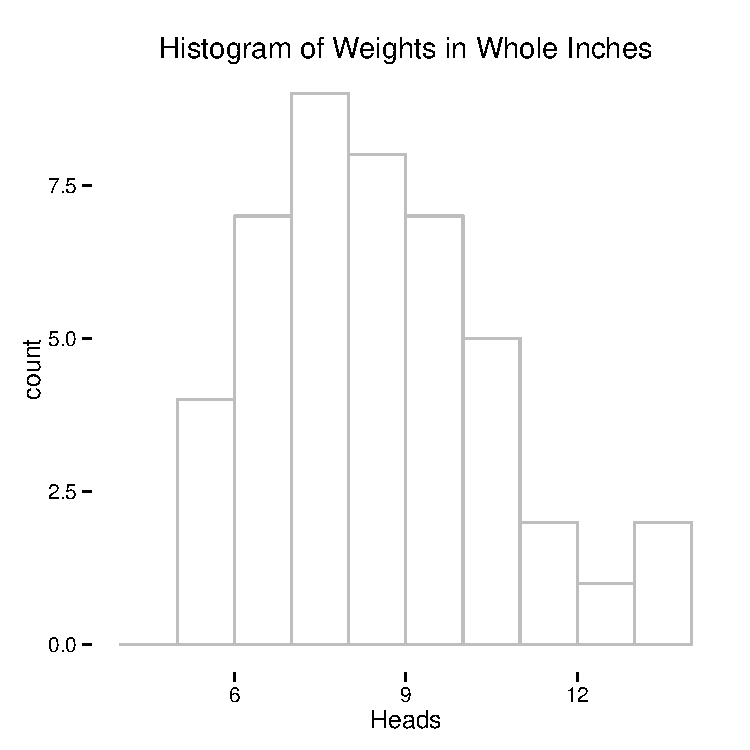
\includegraphics[width=\maxwidth]{figure/graphics-histogram-1} 

}

\caption[Histograms with Frequency Polygon and Ogive (Cumulative Frequency Polygon)]{Histograms with Frequency Polygon and Ogive (Cumulative Frequency Polygon). The Height data set is unimodal, skewed right, with out outlier on the left. }\label{fig:histogram1}
\end{figure}

\begin{figure}

{\centering 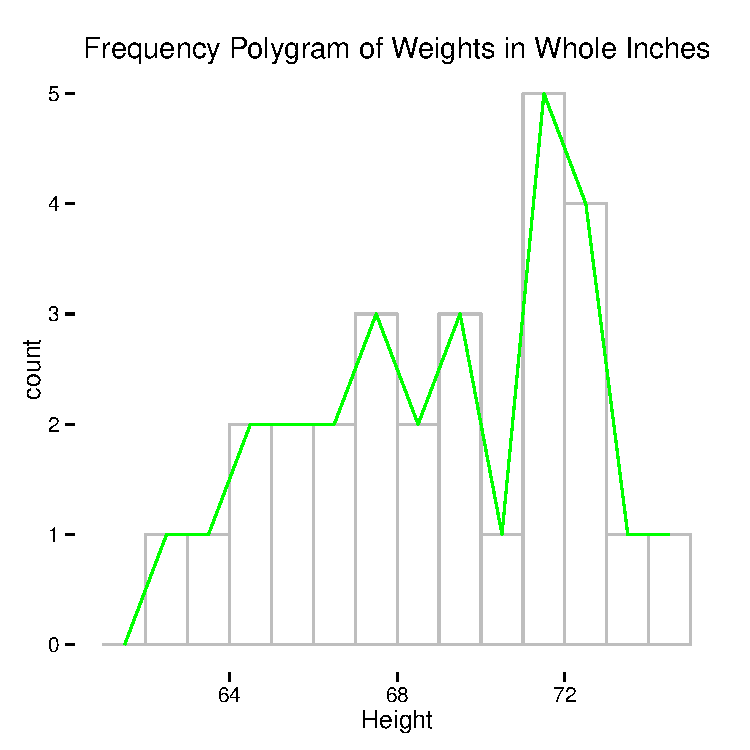
\includegraphics[width=\maxwidth]{figure/graphics-histogram-2} 

}

\caption[Histograms with Frequency Polygon and Ogive (Cumulative Frequency Polygon)]{Histograms with Frequency Polygon and Ogive (Cumulative Frequency Polygon). The Height data set is unimodal, skewed right, with out outlier on the left. }\label{fig:histogram2}
\end{figure}


\end{knitrout}


\begin{knitrout}
\definecolor{shadecolor}{rgb}{0.969, 0.969, 0.969}\color{fgcolor}\begin{figure}[h!]

{\centering 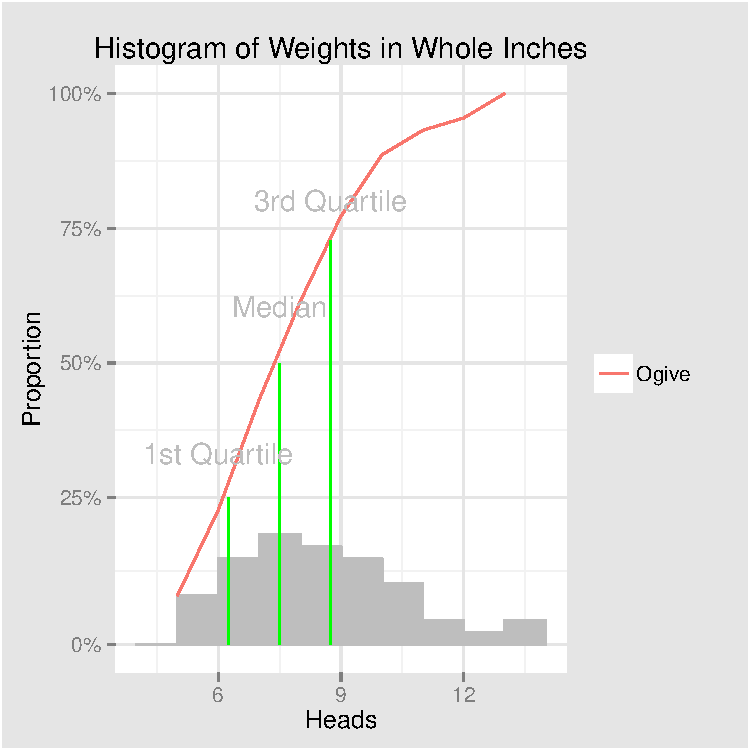
\includegraphics[width=\maxwidth]{figure/graphics-ogive-1} 

}

\caption[Histogram with Ogive (Cumulative Frequency Polygon)]{Histogram with Ogive (Cumulative Frequency Polygon).}\label{fig:ogive}
\end{figure}


\end{knitrout}


\end{document}
